% how to compute the fundamental matrix?
% how to determine communication classes?
% what is the point of computing the entries?
% find ultimate vector
% generalized eigenvalues
\documentclass{hw}
\usepackage{tikz}
\usetikzlibrary{automata,positioning}

\begin{document}
\section*{Bayes Theorem}
\begin{enumerate}
% See the pop vs. soda question
\item Suppose there are 2 cookie jars. Jar A has 10 chocolate chip and 30 plain cookies while jar
B has 20 of each type. We pick a cookie and it turns out to be plain. What is the probability that
we picked out of the jar A?
\begin{quote}
We are trying to find the probability that you chose a cookie from jar A given that you picked a
plain cookie.
\[
P(\text{A}|\text{plain}).
\]
We can find this value by
\[
P(\text{A}|\text{plain})=
{P(\text{A and plain})\over P(\text{plain})}=
{(1/2)(3/4)\over(1/2)(3/4)+(1/2)(20/40)}.
\]
\end{quote}
\item The blue M\&M was introduced in 1995. Before 1995, the ratios of colors was
\begin{gather*}
30\%\text{ brown}\qquad 20\%\text{ yellow}\qquad20\%\text{ red}\\
10\%\text{ green}\qquad 10\%\text{ orange}\qquad10\%\text{ tan}
\end{gather*}
After 1995, the ratios were
\begin{gather*}
24\%\text{ blue}\qquad 20\%\text{ green}\qquad16\%\text{ orange}\\
14\%\text{ yellow}\qquad 13\%\text{ red}\qquad13\%\text{ brown}
\end{gather*}
If we pick an M\&M that turns out to be yellow, what is the probability that the bag came before
1995?
\begin{quote}
We want to find $P(1994|\text{yellow})$. By Bayes theorem, we can find this value by
\[
P(1994|\text{yellow})=
{P(1994\text{ and yellow})\over P(\text{yellow})}=
{(.5)(.2)\over (.5)(.2)+(.5)(.25)}
\]
\end{quote}
\end{enumerate}

\section*{Communication Classes}
\begin{enumerate}
\item What are the communication classes of
\begin{center}
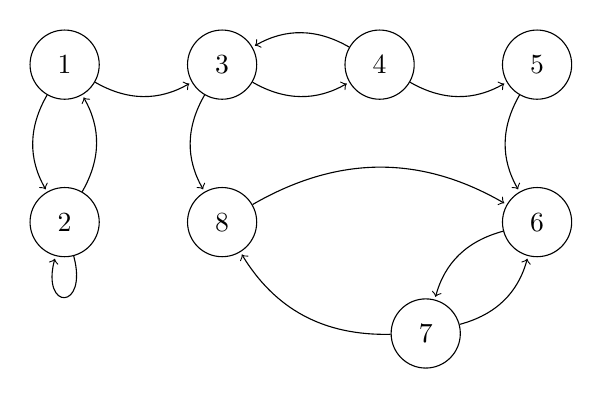
\begin{tikzpicture}[shorten >=1pt,node distance=2cm,on grid,auto]
    \node[state] (one) {1};
    \node[state] (two) [below=of one] {2};
    \node[state] (three) [right=of one] {3};
    \node[state] (four) [right=of three] {4};
    \node[state] (five) [right=of four] {5};
    \node[state] (six) [below=of five] {6};
    \node[state] (seven) [below left=of six] {7};
    \node[state] (eight) [below=of three] {8};

    \path[->]
    (one) edge [bend right] node {} (two)
          edge [bend right] node {} (three)
    (two) edge [bend right] node {} (one)
          edge [loop below] node {} ()
    (three) edge [bend right] node {} (four)
            edge [bend right] node {} (eight)
    (four) edge [bend right] node {} (three)
           edge [bend right] node {} (five)
    (five) edge [bend right] node {} (six)
    (six) edge [bend right] node {} (seven)
    (seven) edge [bend right] node {} (six)
            edge [bend left] node {} (eight)
    (eight) edge [bend left] node {} (six);
\end{tikzpicture}
\end{center}
\begin{quote}
We can find the communication classes by determining if we can move from state $i$ to $j$ and from
state $j$ to $i$.
\end{quote}

\item Consider the matrix
\[
\left(
\begin{array}{c c}
.6 & .4\\
.3 & .7
\end{array}
\right)
\]
\begin{enumerate}
\item How many communication classes are there?
\begin{quote}
There is 1 communication class, since every state is accessible from ever other state.
\end{quote}
\item List the communication class(es).
\begin{quote}
Since there are two states, with one communication class, the communication class is $\{A,B\}$.
\end{quote}
\item Find $\mathbf{\pi}$.
\begin{quote}
To find the $\mathbf{\pi}$ vector, we can solve the system
\[
\begin{cases}
.6\pi_{1}+.3\pi_{2}=\pi_{1}\\
\pi_{1}+\pi_{2}=1
\end{cases}
\]
\end{quote}
\end{enumerate}
\item Consider the model of moving from the city to the suburbs with an initial state.
\[
\begin{array}{c | c c}
& \text{Sub} & \text{City}\\
\hline
\text{Sub} & .95 & .05\\
\text{City} & .03 & .97
\end{array}
\]
\begin{enumerate}
\item What is the probability that a person in 3 years transfers from city to suburb?
\item What number of people in the city will be in the suburbs next year?
\item What is the ultimate number of people in the suburbs? The cities?
\end{enumerate}
\end{enumerate}
\end{document}
